\subsection{Conceptualization of Context}
%\KZ{This is the preliminaries. }

In most of the previous text based image clustering approaches, they use traditional
\emph{bag of words} (BOW) method to represent the context. BOW have drawbacks such as
losing semantics of multi-word expressions (MWEs) and inefficient signals in short texts.
%{\color{red}KQ: an example to explain the drawbacks of BOW and advantage of BOC}
Instead, we propose to represent context as a weighted list of higher level concepts,
in a process known as \emph{Conceptualization}.

%Comparing with BOW, conceptualization has two main advantages. One is that conceptualization
%represents context via phrases rather than words which can express human's meaning
%better. Also, one phrase may mean rather different from its word components. The other
%is that conceptualization
%represent context by fixed-meaning concept, while BOW representation is usually ambiguous.
%That is to say, conceptualization is more accurate than BOW, which can improve the
%result of text based image clustering better.

%\subsection{Wikipedia Conceptualization}
Wikipedia is a rich and comprehensive knowledge source of concepts.
It contains over 3 million concepts (or entities) in a version dated May 2011 used
in this paper.
Each concept (e.g. {\em Mr. Bean} or {\em Phaseolus vulgaris}) has a corresponding article
which describes the meaning of this concept.
Given a plain text, the goal of conceptualization based on Wikipedia is to use a set of
Wikipedia concepts to represent it. To achieve this, we need to recognize the MWEs
(a.k.a. terms) in the plain text and then disambiguate them
by identifying the best sense of each
term and linking it to a corresponding Wikipedia article. This process is known as
\emph{wikification} \cite{MihalceaC07}. %\figref{fig:screen-bear} shows an example of Wikification. ``Polar
%Bear'' is assigned the Wikipedia concept ``Snow Patrol'', which is the name of a rock band.
%However, ``Polar'' and ``Bear'' both have no relation to music, showing that BOW may
%sometimes mis-represent the context.
%
%\begin{figure}
%\centering
%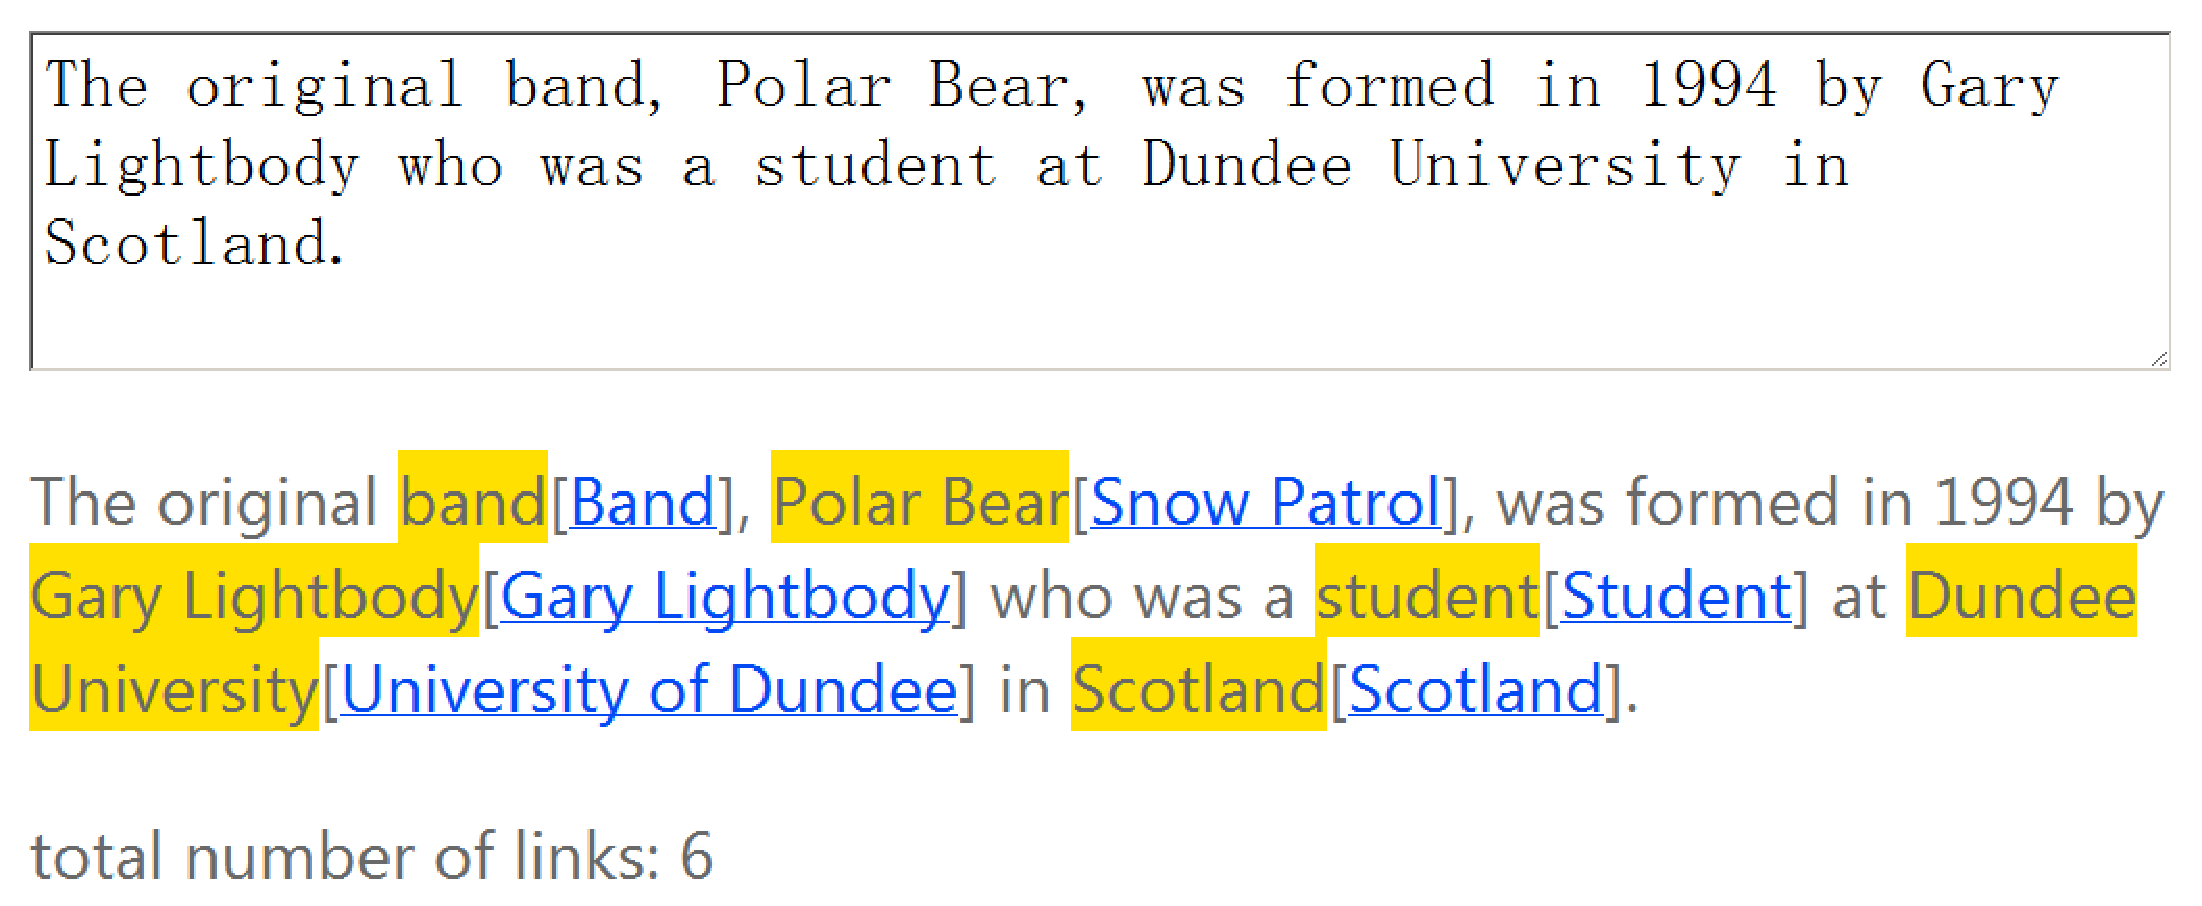
\epsfig{file=screen-bear.eps,width=\columnwidth}
%\caption{An Example of Wikification}
%\label{fig:screen-bear}
%\end{figure}

%We conceptualize plain texts in three steps: \emph{Wikification},
%\emph{Ranking}, and \emph{Extension}.
%\textbf{Wikification} is a hot topic in recent years.
%Systems of Wikification assign a link from
%nouns in plain text to a corresponding Wikipedia article URL.
%It is a kind of noun phrase sense disambiguation.
%We use Wikification to detect Wikipedia concepts
%which can explicitly point out the exact sense of ambiguous phrases in the text.
%Unlike the previous works\cite{cucerzan2007large}\cite{kulkarni2009collective}\cite{ferragina2010tagme},

In this paper, we adopt a wikification approach which is based on
concept co-occurrence.
We collect co-occurrence frequencies between concepts by
scanning Wikipedia corpus. We also apply an iterative process
bootstrapping Wikipedia corpus to collect more co-occurrence information. With enough
co-occurrence information, the wikification process finds the best combination
of concepts which gives the highest co-occurrence frequency among them.
It then assign these concepts to corresponding terms.
If we have $N$ terms, each term has $k$ candidate senses,
the total candidate combinations will be $k^N$. Attempting all these combinations is
prohibitive in time.
To balance accuracy and complexity, we use a sliding window to
narrow the number of terms considered each time.
The following example demonstrates this idea.

Suppose the context contains five terms: $A$, $B$, $C$, $D$ and $E$. The sets of their candidate sense
are denoted as $\{a_i\}$, $\{b_i\}$, $\{c_i\}$, $\{d_i\}$ and $\{e_i\}$.
Let the window size be 3.
In the first step of the wikification process, since the window size is three,
we just consider three terms, $A$, $B$ and $C$.
By picking one sense from $\{a_i\}$, $\{b_i\}$ and $\{c_i\}$ respectively,
we form several sense combinations. We assign a score to each combination by calculating the sum of
the co-occurrence frequency of each pair of concepts in that combination. Assume that
$a_1$, $b_2$ and $c_2$ is the best sense combination with a score of 15,
we store this result in a concept-score pair form,
$\langle a_1,15\rangle$ and $\langle b_2,15\rangle$. Then we slide the window forward
by one term.  This time the terms being considered are $B$, $C$ and $D$.
Similar to the previous step, we calculate
the best combination and then store the result. After handling $C$, $D$ and $E$,
we aggregate the result in each step to get the final wikification result.
Given the concept-score pairs in the three steps as follow:

\begin{itemize}
\item {$\langle a_1,15\rangle$ $\langle b_2,15\rangle$ $\langle c_2,15\rangle$}
\item {$\langle b_2,18\rangle$ $\langle c_3,18\rangle$ $\langle d_1,18\rangle$}
\item {$\langle c_2,13\rangle$ $\langle d_2,13\rangle$ $\langle e_2,13\rangle$}
\end{itemize}

we combine the records with the same concept by summing the scores.
Thus, $\langle c_2,15\rangle$ and $\langle c_2,13\rangle$
are combined to be $\langle c_2,28\rangle$.
Finally, we assign the concept with the highest score to each term.
The final wikification result for this example is: $a_1$,$b_2$,$c_2$,$d_1$,$e_2$.

%{\color{red}KQ: an example of Wikification}

%\textbf{Ranking} of concepts is to assign an ``importance'' measure to Wikipedia concepts
%in the given text. \emph{TF-IDF} is a very common metric of measuring importance.
%Similar to \emph{TF-IDF}, we use \emph{CF-IDF}(concept frequency and concept inverse document frequency) to
%assign a score to each concept. To obtain the concept \emph{IDF},
%we scan all of the articles in Wikipedia corpus, and for each concept, we count the number of documents in
%which the concept appears as a link. Consider that, many terms are not linked in the original Wikipedia
%data. To hold the statistical characteristics of \emph{IDF} score, we add links to the unlinked terms in Wikipedia.
%{\color{red}KQ:Describe the method of adding links to Wikipedia}
%First of all, we scan the initial Wikipedia corpus to build a co-occurrence matrix. Each cell in the matrix
%stores the co-occurrence frequency of two Wikipedia concepts. We start from this matrix to add links to
%Wikipedia. For each unlinked term, which has several ambiguous senses, we calculate a conditional probability
%each sense of it that can be used to disambiguate this term, based on the co-occurrence frequency between
%each candidate sense and the senses of the unlinked term's linked neighbours. The sense with the highest
%probability will be picked as the sense of the unlinked term, if the probability is higher than a threshold.
%Then we link this term to the corresponding Wikipedia page. Adding links to Wikipedia corpus will bring us
%more co-occurrence information, which will help us to disambiguate more unlinked terms. We continue this
%iterative process until no more linked can be added.
%
%Finally, the \emph{CF-IDF} is compute in the following way:
%\begin{equation}
%CF-IDF(c, d) = cf(c, d) * log\frac{N}{df(c)}
%\end{equation}
%where $c$ is a Wikipedia concept, $d$ is the given document and $N$ is the total number of
%Wikipedia articles. $cf(c,d)$ stands for frequency of $c$ in $d$, and $df(c)$ is numbers of Wikipedia articles
%in which $c$ occurs.
%
%\textbf{Expansion}
%In many cases, the context of an image is limited. {\color{red}KQ: add examples}
%We expand the concepts we obtained from Wikification, to get more information.
%Expand concepts will have risks of expanding the noise. We only expand top K concepts
%ranked by \emph{CF-IDF} score, to control the expansion of noise. We present the top K concepts,
%using links in the Wikipedia article of the concepts. {\color{red}KQ: example of concepts expansion}


%\subsection{Probase Conceptualization}
%Probase is a probabilistic taxonomy built from \emph{Hearst Pattern}. Entries in \emph{Probase} can be
%an instance(\emph{hyponym}) or a class(\emph{hypernym}). For example, \emph{kiwi} is an instance of
%\emph{bird}, while \emph{bird} is one of the classes of \emph{kiwi}. From \emph{Probase}, we can know
%the probability of \emph{kiwi} to be a \emph{fruit} is 29.09\%, while \emph{kiwi} to be a \emph{bird}
%with probability of 1.95\%. Besides \emph{fruit} and \emph{bird}, the classes of \emph{kiwi} contains
%concepts like \emph{food}, \emph{flightless bird}, \emph{species}, etc. The sum of $P(c|kiwi)$ is 1, where
%$c$ stands for one of the classes of kiwi. The approach of conceptualize short text using Probase is
%introduced by Yangqiu\cite{Yangqiu2011}. The idea of conceptualization based on \emph{Probase} is to model as a
%Na\"{i}ve Bayesian model. The probability of a concept given a text is computed in the following way:
%\begin{equation}
%P(c_k|E)\propto P(c_k)\prod_{i=1}^{N}{P(e_i|c_k)}
%\end{equation}
%where $P(e_i|c_k)$ is known in the taxonomy, $e_i$ is the instances detected from the text, and $c_k$ is
%a class of any of the instances. Like Wikification, using this model, we can obtain a distribution(weighted vector)
%on Probase concept space of the text.

